\documentclass[tikz, border=1mm]{standalone}
\usepackage{tikz} 
\usetikzlibrary{arrows.meta}
\usepackage{pgfplots}

\pgfplotsset{compat=1.18}

\begin{document}

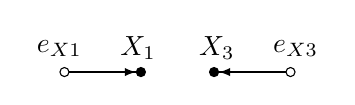
\begin{tikzpicture}

    % dag_bb1
    \node at (-2,0) {$e_{X1}$};
    \node at (-1,0) {$X_{1}$};
    \node at (0,0) {$X_{3}$}; 
    \node at (1,0) {$e_{X3}$};

    %\draw[black, fill=black] (-1,-0.3) circle(1.6pt);
    %\draw[black, fill=black] (0,-0.3) circle(1.6pt);
    \draw[{Circle[open]}-{latex}{Circle}](-2,-0.3) to (-0.9,-0.3); % eX -> X (circle)
    \draw[{Circle[open]}-{latex}{Circle}](1,-0.3) to (-0.1,-0.3); % eY -> Y (circle)
    %\draw[{Circle}-{latex}{Circle}](-1.05,-0.3) to (0.05,-0.3); % X -> Y (circle)
    
\end{tikzpicture}

\end{document}
